\documentclass{beamer}
\setbeamertemplate{footline}[page number]
\date{}
\author{}
\institute{}

%%%%%%% Put these names back in the final version 
%\\Aswathy Rajendra Kurup\\Meenu Ajith}
%\institute{Department of Electrical and Computer Engineering\\The University of New Mexico}
\setbeamercovered{transparent}
\usepackage{setspace}
\usepackage{array}
\usepackage[T1]{fontenc}
\usepackage{graphicx}
\usepackage{amsmath}
\usepackage{amsfonts}
\usepackage{amssymb}
\usepackage{makeidx}
\usefonttheme{serif}
\usepackage{multirow}
\usepackage{booktabs} 
\usepackage{rotating}
\usepackage{color}
\usepackage{float}
\usepackage[latin1]{inputenc}
\usepackage[english]{babel}
\usepackage{amsmath}
\usepackage{amsfonts}
\usepackage{eurosym}
\usepackage{rotating}
\usepackage{multicol}
\usepackage{pythonhighlight}
\usepackage[normalem]{ulem}
\newcommand{\ba}{{\bf a}}
\newcommand{\bb}{{\bf b}}
\newcommand{\bc}{{\bf c}}
\newcommand{\bd}{{\bf d}}
\newcommand{\be}{{\bf e}}
\newcommand{\bbf}{{\bf f}}
\newcommand{\bg}{{\bf g}}
\newcommand{\bh}{{\bf h}}
\newcommand{\bi}{{\bf i}}
\newcommand{\bk}{{\bf k}}
\newcommand{\bl}{{\bf l}}
\newcommand{\bm}{{\bf m}}
\newcommand{\bn}{{\bf n}}
\newcommand{\bo}{{\bf o}}
\newcommand{\bp}{{\bf p}}
\newcommand{\bq}{{\bf q}}
\newcommand{\br}{{\bf r}}
\newcommand{\bs}{{\bf s}}
\newcommand{\bt}{{\bf t}}
\newcommand{\bu}{{\bf u}}
\newcommand{\bv}{{\bf v}}
\newcommand{\bw}{{\bf w}}
\newcommand{\bx}{{\bf x}}
\newcommand{\by}{{\bf y}}
\newcommand{\bz}{{\bf z}}

\newcommand{\bA}{{\bf A}}
\newcommand{\bB}{{\bf B}}
\newcommand{\bC}{{\bf C}}
\newcommand{\bE}{{\bf E}}
\newcommand{\bG}{{\bf G}}
\newcommand{\bH}{{\bf H}}
\newcommand{\bI}{{\bf I}}
\newcommand{\bK}{{\bf K}}
\newcommand{\bL}{{\bf L}}
\newcommand{\bM}{{\bf M}}
\newcommand{\bO}{{\bf O}}
\newcommand{\bQ}{{\bf Q}}
\newcommand{\bR}{{\bf R}}
\newcommand{\bS}{{\bf S}}
\newcommand{\bT}{{\bf T}}
\newcommand{\bV}{{\bf V}}
\newcommand{\bW}{{\bf W}}
\newcommand{\bX}{{\bf X}}
\newcommand{\bY}{{\bf Y}}
\newcommand{\bZ}{{\bf Z}}
\newcommand\uptocnt{\stackrel{\mathclap{\normalfont\mbox{c}}}{\propto}}
\newcommand{\bpt}{{\bf pt}}
\newcommand{\bpl}{{\bf pl}}
\newcommand{\bdp}{{\bf dp}}
\newcommand{\btemp}{{\bf temp}}

\newcommand{\bmu}{{\boldsymbol \mu}}
\newcommand{\bSigma}{{\boldsymbol \Sigma}}
\newcommand{\bsigma}{{\boldsymbol \sigma}}
\newcommand{\bvarPhi}{{\boldsymbol \varPhi}}
\newcommand{\bvarphi}{{\boldsymbol \varphi}}
\newcommand{\bPhi}{{\boldsymbol \Phi}}
\newcommand{\bdelta}{{\boldsymbol \delta}}
\newcommand{\bZero}{{\bf 0}}
\newcommand{\bOne}{{\bf 1}}
\newcommand{\balpha}{{\boldsymbol \alpha}}
\newcommand{\bAlpha}{{\boldsymbol A}}
\newcommand{\btheta}{{\boldsymbol \theta}}

\newcommand{\softmax}{\text{softmax}}
\newcommand{\diag}{\text{diag}}
\newcommand{\sinc}{\mathrm{sinc}}
\newcommand{\argmin}{\mathop{\mathrm{argmin}}}
\newcommand{\infl}{\eta}
\newcommand{\Ind}{\mathrm{I}}
\newcommand{\Real}{\mathbb R}
\newcommand{\Intg}{\mathbb Z}
\newcommand{\Complex}{\mathbb C}
\newcommand{\Natural}{\mathbb N}
\newcommand{\Fourier}[1]{\mathcal{F} \{#1\}}
%\newcommand{\ii}{\mathbbm{i}}
\newcommand{\bphi}{\boldsymbol{\mathit{\phi}}}

\newcommand{\hs}{\hspace{2pt}}
\newcommand{\sign}{\text{sign}}
\author{Manel Mart\'inez-Ram\'on\\Meenu Ajith\\Aswathy Rajendra Kurup}

\usetheme{Madrid}
\usecolortheme{beaver}
\usepackage{tikz}
\usetikzlibrary{fit,arrows,calc,positioning}
\usepackage{listings}
\usepackage{xcolor}
\usepackage{emerald} 
\usepackage[T1]{fontenc} 
\usepackage{verbatim}
\usepackage{graphicx}
\usepackage{epsfig}
\usepackage{psfrag}
\usepackage[english]{babel}
\usepackage{listings}
\usepackage{courier}
\usepackage{color}
 \usepackage{vwcol} 
 \usepackage[english]{babel} % To obtain English text with the blindtext package
\usepackage{blindtext}
\definecolor{codegreen}{rgb}{0,0.6,0}
\definecolor{codegray}{rgb}{0.5,0.5,0.5}
\definecolor{codepurple}{rgb}{0.58,0,0.82}
\definecolor{backcolour}{rgb}{0.95,0.95,0.92}

\lstdefinestyle{mystyle}{
  backgroundcolor=\color{backcolour},   commentstyle=\color{codegreen},
  keywordstyle=\color{magenta},
  numberstyle=\tiny\color{codegray},
  stringstyle=\color{codepurple},
  basicstyle=\ttfamily\footnotesize,
  breakatwhitespace=false,         
  breaklines=true,                 
  captionpos=b,                    
  keepspaces=true,                 
  numbers=left,                    
  numbersep=5pt,                  
  showspaces=false,                
  showstringspaces=false,
  showtabs=false,                  
  tabsize=2
}
\lstset{style=mystyle}

%% Stuff for movies

% %\newcommand{\bt}{{\bf t}}
% \newcommand{\br}{{\bf r}}
% \newcommand{\bs}{{\bf s}}
% \newcommand{\by}{{\bf y}}
% \newcommand{\bz}{{\bf z}}
% \newcommand{\bx}{{\bf x}}
% \newcommand{\bw}{{\bf w}}
% \newcommand{\be}{{\bf e}}
% \newcommand{\bbf}{{\bf f}}
% \newcommand{\bb}{{\bf b}}
% \newcommand{\bd}{{\bf d}}
% \newcommand{\bA}{{\bf A}}
% \newcommand{\bB}{{\bf B}}
% \newcommand{\bL}{{\bf L}}
% \newcommand{\bM}{{\bf M}}

% \newcommand{\bC}{{\bf C}}
% \newcommand{\bI}{{\bf I}}
% \newcommand{\bK}{{\bf K}}
% \newcommand{\bk}{{\bf k}}
% \newcommand{\bT}{{\bf T}}
% \newcommand{\bV}{{\bf V}}
% \newcommand{\bW}{{\bf W}}
% \newcommand{\bX}{{\bf X}}
% \newcommand{\bY}{{\bf Y}}
% \newcommand{\bZ}{{\bf Z}}
% \newcommand{\bm}{{\bf m}}
% \newcommand{\bpt}{{\bf pt}}
% \newcommand{\bpl}{{\bf pl}}
% \newcommand{\bdp}{{\bf dp}}
% \newcommand{\btemp}{{\bf temp}}
% \newcommand{\bl}{{\bf l}}
% \newcommand{\bu}{{\bf u}}
% \newcommand{\bmu}{{\boldsymbol \mu}}
% \newcommand{\bSigma}{{\boldsymbol \Sigma}}
% \newcommand{\bLambda}{{\boldsymbol \Lambda}}

% \newcommand{\bsigma}{{\boldsymbol \sigma}}
% \newcommand{\bvarphi}{{\boldsymbol \varPhi}}
% \newcommand{\btheta}{{\boldsymbol \theta}}
% \newcommand{\bZero}{{\bf 0}}
% \newcommand{\balpha}{{\boldsymbol \alpha}}
% \newcommand{\bpi}{{\boldsymbol \pi}}
% \newcommand{\bxi}{{\boldsymbol \xi}}
% \newcommand{\bdelta}{{\boldsymbol \delta}}
\lstset{
	language=Python,
	basicstyle=\footnotesize\ttfamily\color{black},
	commentstyle = \footnotesize\ttfamily\color{red},
	keywordstyle=\footnotesize\ttfamily\color{blue},
	stringstyle=\footnotesize\ttfamily\color{black},
%	columns=fixed,
%	numbers=left,    
	numberstyle=\tiny,
	stepnumber=1,
	numbersep=5pt,
	tabsize=1,
	extendedchars=true,
	breaklines=true,            
	frame=b,         
	showspaces=false,
	showtabs=true,
	xleftmargin=6pt,
	framexleftmargin=6pt,
	framexrightmargin=2pt,
	framexbottommargin=4pt,
	showstringspaces=false      
}

\lstloadlanguages{
         Python
}

%\graphicspath{ {./images/} }  % Figures path - used in graphicx

%\selectcolormodel{cmyk}

\mode<presentation>

\newcommand{\dred}{darkred!90!black}
\newcommand{\written}{\ECFJD\textcolor{cyan!50!white}}
\newcommand{\hlight}{\textcolor{\dred}}
\newcommand{\Ex}{\textcolor{\dred}{Ex. }}

% remove navigation symbols in full screen mode
\setbeamertemplate{navigation symbols}{}  
\setbeamertemplate{blocks}[rounded][shadow=false]
\setbeamercolor{note page}{fg=black}

\setbeamercolor{title}{fg=\dred}
\setbeamercolor{frametitle}{fg=white}
\setbeamercolor{frametitle}{bg=\dred}
\setbeamercolor{structure}{fg=black,bg=white}
\setbeamercolor{background canvas}{bg=white,fg=black}
\setbeamercolor{normal text}{fg=black,bg=white}
\setbeamercolor{item}{fg=red!80!black,bg=white!}
\addtobeamertemplate{block begin}{\setbeamercolor{block title}{fg=white,bg=\dred}
\setbeamercolor{block body}{fg=white,bg=gray}}{}


\usepackage{algorithm,algorithmic}
\usepackage[algo2e]{algorithm2e} 
%\title{Lesson 1.1}
\title{1. Feedforward neural networks}
\subtitle{1.3b. The Backpropagation algorithm (2)}


\addtobeamertemplate{frametitle}{}


\begin{document}

\maketitle

\begin{frame}{Gradient  with respect to hidden  weights}

\begin{itemize}
\item Using the same reasoning as before, we compute the gradient of the cost function $J_{ML}(\by,\bbf(\bx))$ with respect to weight $w^{(L-1)}_{i,j}$:
\begin{equation}
    \frac{d}{dw_{i,j}^{(L-1)}} J_{ML}\left(
    \by,\underbrace{\bo\left({\bW^{(L)}}^\top\bphi\left({\bW^{(L-1)}}^\top\bh^{(L-2)}\right)\right)}_{\bbf(\bx)}
    \right)
\end{equation}
\item First, we determine what elements are connected to $w_{i,j}^{(L-1)}$, and this can be done graphically.

\end{itemize}
\end{frame}
\begin{frame}
\begin{multicols}{2}
\begin{center}
    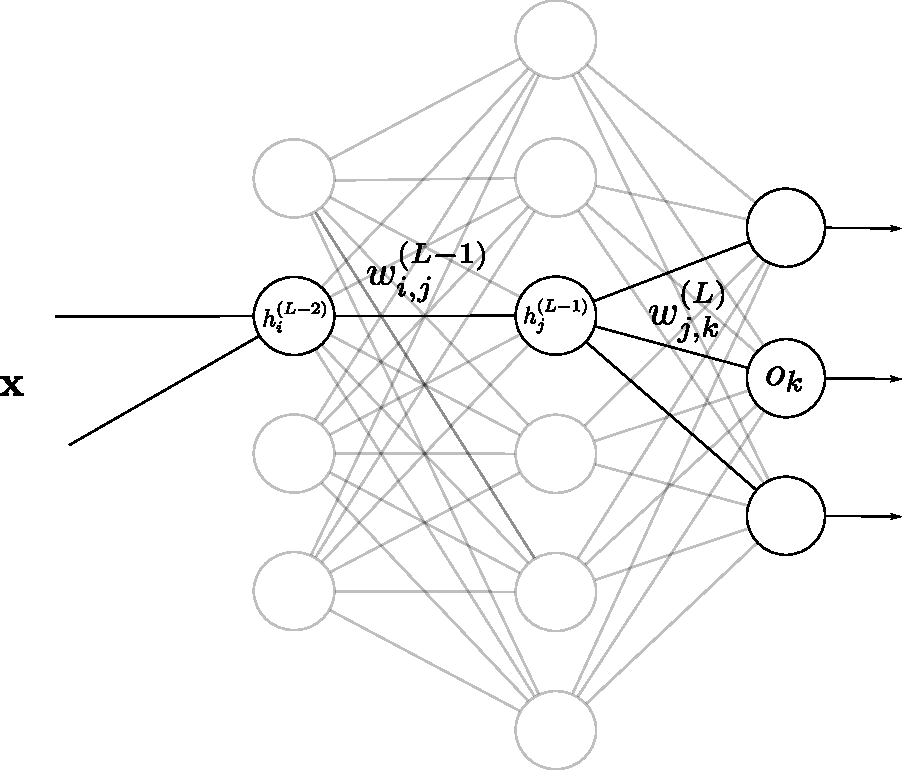
\includegraphics[scale=0.32]{Module 1 (NN)/pics/backprop.pdf}
    \end{center}
    
\columnbreak
~\\
\begin{itemize}
\item Elements involved in the computation of the derivative with respect to $w_{i,j}^{(L-1)}$:
\begin{itemize}
\item Weights $w_{j,k}^{(L)}$ and outputs $o_k$.
\item Node $h_j^{(L-1)}$.
\item Node $h_i^{(L-2)}$.
\end{itemize}
\end{itemize}
\end{multicols}
\end{frame}

\begin{frame}{Chain rule}{Hidden layer}

\begin{itemize}
    \item Specifically, the elements of the chain are
\begin{equation}\label{eq:elements_chain}
    \begin{array}{rl}
        o_k = o(z_k^{(L)}), & z_k^{(L)} = \bw_k^{(L)}\bh^{(L-1)},~\forall k \\
    h_j^{(L-1)}=\phi\left(z_j^{(L-1)}\right),
        &z_j^{(L-1)} = \bw_j^{(L-1)}\bh^{(L-2)} \\
    \end{array}
\end{equation}
where  $\bw_j^{(L-1)}$ contains the element of interest  $w_{i,j}^{(L-1)}$. 



\item We can compute the derivative with respect to $w_{i,j}^{(L-1)}$:  

\begin{equation}\label{eq:backprop_L-1_first}
    \frac{d}{dw_{i,j}^{(L-1)}}   J_{ML}(\by,\bbf(\bx)) = \sum_{k}
    \underbrace{\frac{\delta J_{ML}}{do_k}\frac{do_k}{dz_k^{(L)}}}_{\delta_k^{(L)}}
    \underbrace{\frac{dz_k^{(L)}}{dh_{j}^{(L-1)}}}_{w_{j,k}^{(L)}}
    \underbrace{\frac{dh_j^{(L-1)}}{dz_j^{L-1}}}_{\phi'}
    \underbrace{\frac{dz_j^{(L-1)}}{dw_{i,j}^{(L-1)}}}_{h_i^{L-2}}
\end{equation}
\end{itemize}
\end{frame}
\begin{frame}{Chain rule}{Hidden layer}
\begin{itemize}
\item Taking into account the expressions in Eqs. \eqref{eq:elements_chain} and \eqref{eq:backprop_L-1_first}, this turns into equation 

\begin{equation}\label{eq:backprop_L-1}
    \frac{d}{dw_{i,j}^{(L-1)}}   J_{ML}(\by,\bbf(\bx)) =\underbrace{\sum_{k}
    \delta_k^{(L)}w_{k,j}^{(L)}\phi'\left(z^{(L-1)}_j\right)}_{\delta_j^{L-1}}
    h^{L-2}_i=h^{(L-2)}_i\delta_j^{(L-1)}
\end{equation}
\item Expression $\sum_{k} \delta_k^{(L)}w_{k,j}^{(L)}$ is the element $j$ of vector $\bW^ {(L)}{\boldsymbol \delta}^{(L)}$
\item This vector is elementwise multiplied with the elements of $\bphi'\left(\bz^{(L-1)}\right)$. 
\end{itemize}

\end{frame}
\begin{frame}{Weight update}{Hidden layer}
    \begin{itemize}
        \item In summary, from 

\begin{equation}\nonumber 
    \frac{d}{dw_{i,j}^{(L-1)}}   J_{ML}(\by,\bbf(\bx)) =\sum_{k}
    \delta_k^{(L)}w_{k,j}^{(L)}\phi'\left(z^{(L-1)}_j\right)
    h^{L-2}_i=h^{(L-2)}_i\delta_j^{(L-1)}
\end{equation}
\item we define 
        \begin{equation}
    {\boldsymbol \delta}^{(L-1)} = \bW^ {(L)}{\boldsymbol \delta}^{(L)}\odot \phi'\left(\bz^{(L-1)}\right)
\end{equation}
\item  and 
\begin{equation}
 \nabla_{\bW^{L-1}}J_{ML}\left(\by,\bbf\left(\bx\right)\right)={\bh^{(L-2)}} {\boldsymbol \delta}^{(L-1)^\top} 
\end{equation}


\item Finally

\begin{equation}
    \bW^{(L-1)} \leftarrow     \bW^{(L-1)}  - \mu  {\bh^{(L-2)}} {\boldsymbol \delta}^{(L-1)^\top}
\end{equation}  
\end{itemize}
\end{frame}

\begin{frame}{Weight update}{Hidden layer}
    \begin{itemize}
        \item The process can be iterated down to the input layer, with the same result, and therefore the update of weight matrix $\bW^{(l-1)}$ is 
\begin{equation}\label{eq:bp_update}
    \bW^{(l-1)} \leftarrow \bW^{(l-1)} - \mu   {\bh^{(l-2)}} {{\boldsymbol \delta}^{(l-1)}}^\top
\end{equation}
where
\begin{equation}\label{eq:general_error_term}
    {\boldsymbol \delta}^{(l-1)} = \bW^ {(l)}{\boldsymbol \delta}^{(l)}\odot
    \phi'\left(\bz^{(l-1)}\right)
\end{equation}

where to start and end the process, we need
\begin{equation}
\begin{split}
\bdelta^{(L)} & = \nabla_{\bo}J_{ML}(\by,\bo) \odot \bo'\\
\bh^{(0)}&=\bx  ~~\text{(Input layer)}
\end{split}
\end{equation}
\end{itemize}
\end{frame}

\end{document}